\newlength{\shiftx}
\newlength{\shifty}
\setlength{\shiftx}{-500mm}
\setlength{\shifty}{11.1mm}

\begin{myblock2}{\Large Access through the Collaboratory \phantom{\Huge $\beta$}}
	
	% \vspace{+5.cm}
	% \vspace{-23.8mm}\hspace{+25mm}\tikzmark{ptd}
	% \vspace{+23.8mm}\hspace{-25mm}
	% \vspace{-39.8mm}\hspace{+91mm}\tikzmark{ptf}
	% \vspace{+39.8mm}\hspace{-91mm}
	% \vspace{-.3cm}
	
	\begin{figure}[t]
		\centering
		\adjincludegraphics[trim={0 {.02\height} 0 {.00\height}}, clip, width=1.0\textwidth]{\imgpath/picture-collab-neutre}
		% 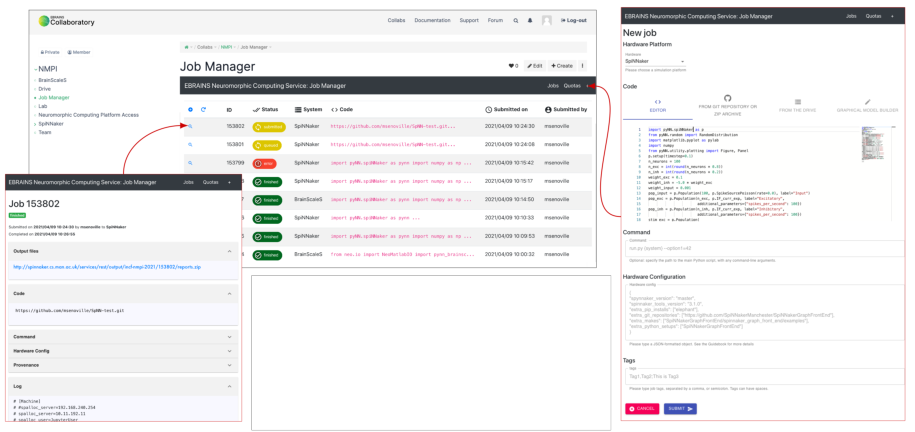
\includegraphics[width=1.\textwidth,angle=00]{\imgpath/picture-collab-neutre}
	\end{figure}
	\vspace{-130mm}
	\begin{columns}[t]
		\column{.24\textwidth}
		            
		\column{.35\textwidth}
		\begin{normalsize}
			\justify
			\setlength{\parindent}{0mm} 
			The Neuromorphic Job Manager is a web based app providing a graphical interface for submitting jobs
			to the BrainScaleS and SpiNNaker systems and for retrieving job results,
			with detailed provenance metadata including full log files.\\[2mm]
			\justify 
			As a Community app the Job Manager is integrated into the EBRAINS Collaboratory, which aims to be a workspace for scientific collaboration,
			sharing and collaboration around data, software and services.    
			\\[24mm]
			\phantom{-}
		\end{normalsize}
		\column{.3\textwidth}
		
	\end{columns}
	    
	% \begin{tikzpicture}[remember picture,overlay]
	% 	\node[xshift=\shiftx+0cm,yshift=\shifty+0cm] at (current page.center) {
	% 		\adjincludegraphics[trim={0 {.20\height} 0 {.00\height}}, clip, width=0.6\textwidth, cfbox=black 0.1pt 0pt 0pt]{\imgpath/screenshot/collab/fichier-57.png}
	% 	};
	% \end{tikzpicture}
	% \begin{tikzpicture}[remember picture,overlay]
	% 	\node[xshift=\shiftx+45mm,yshift=\shifty+-0.06\textheight] at (current page.center) {
	% 		\adjincludegraphics[trim={0 {.2\height} 0 {.00\height}}, clip, width=0.3*25cm, cfbox=white 0.0pt 0pt 0pt]{\imgpath/screenshot/list/fichier-3-wo-space.png}
	% 	};
	% \end{tikzpicture}
	% \begin{tikzpicture}[remember picture,overlay,
	% 	arrow/.style={red!80!black,thin,->,>=latex,outer sep=-.5cm}]
	% 	\node[xshift=0.373\textwidth,yshift=-0.024\textheight](jobcreation) at (current page.center) {
	% 		\adjincludegraphics[trim={0 0 0 {.004\height}}, clip, width=0.3\textwidth, cfbox=red!80!black 0.1pt 0pt -2.5pt]{\imgpath/screenshot/create/fichier-30.png}
	% 	};
	% 	\draw[arrow]
	% 	(jobcreation) to[out=180,in=0] ([yshift=6.7mm]{pic cs:ptf}); 
	% \end{tikzpicture}
	% \begin{tikzpicture}[remember picture,overlay,
	% 	arrow/.style={red!80!black,thin,->,>=latex,outer sep=-.5cm}]
	% 	\node[xshift=-0.4\textwidth,yshift=-0.19\textheight](jobdetails) at (current page.center) {
	% 		\adjincludegraphics[trim={0 {.3\height} 0 {.000\height}}, clip, width=0.25\textwidth, cfbox=red!80!black 0.1pt 0pt -2.5pt]{\imgpath/screenshot/details/fichier-9.png}
	% 	};
	% 	\draw[arrow]
	% 	(jobdetails) to[out=90,in=180] ([yshift=-0.mm]{pic cs:ptd}); 
	% \end{tikzpicture}
	
\end{myblock2}